\documentclass[11pt]{article}
\usepackage[T1]{fontenc}
\usepackage[utf8]{inputenc}
\usepackage{mathptmx}
\usepackage[margin=1in]{geometry}
\usepackage{setspace}\onehalfspacing
\usepackage{microtype,graphicx,booktabs,tabularx,threeparttable,xcolor}
\usepackage[labelfont=bf,font=small]{caption}
\usepackage{enumitem}\setlist{itemsep=2pt,topsep=4pt}
\usepackage[hidelinks]{hyperref}
\usepackage{newunicodechar}
\newunicodechar{−}{\ensuremath{-}}
\newunicodechar{κ}{\ensuremath{\kappa}}
\newunicodechar{±}{\ensuremath{\pm}}
\newunicodechar{×}{\ensuremath{\times}}
\newunicodechar{†}{\textdagger}
\newunicodechar{◆}{\ensuremath{\diamond}}
\newunicodechar{§}{\S}
\providecommand{\tightlist}{\setlength{\itemsep}{2pt}\setlength{\parskip}{0pt}}
\setlength{\parskip}{0pt}
\renewcommand{\floatpagefraction}{0.75}
\renewcommand{\topfraction}{0.85}
\title{\textbf{Protection Follows the Label: How Large Language Model Résumé Screeners Turn the Motherhood Penalty into a Caregiver Penalty}}
\author{Yuxin Hou\\\small Princeton University}
\date{\small Draft, October 31, 2026}
\begin{document}
\maketitle
\begin{abstract}\noindent Large language models (LLMs) now screen job applicants, and their
developers train them not to treat people differently by gender. We ask
what such systems do with the signals that make up the motherhood
penalty. On a résumé, motherhood bundles a protected category (being a
woman) with signals that are correlated with gender but not protected as
such: an interruption in employment and visible family responsibilities.
We propose that in aligned models, \emph{protection follows the label}:
the more directly a signal names a protected category, the more
carefully models handle it, while correlated signals are penalized
freely. Study 1, an audit of widely used models (616,419 decisions, 28
occupations), unbundles the signal on otherwise identical résumés and
places each component along this gradient. Signals of caregiving carry a
large penalty, for mothers and fathers alike, visible only when
applicants are compared: a parent returning from leave wins a
head-to-head choice against an equally qualified childless applicant 19
to 31 percent of the time. The penalty is unchanged when all gender
information is removed. Explicitly named gender elicits small,
vendor-specific behavior---correction toward women or parity---rather
than a penalty. An instruction that names caregiving gaps reduces the
gap penalty but not the penalty on family signals it leaves unnamed.
Study 2, planned, tests whether the gradient emerges with alignment by
comparing the same open-weight model before and after post-training.
Because women carry caregiving signals more often than men, a screener
that protects the label can reproduce the motherhood penalty in effect.\end{abstract}
\vspace{0.5em}
\hypertarget{introduction}{%
\section{Introduction}\label{introduction}}

Mothers pay a price in the labor market that fathers do not. They earn
less than comparable childless women (Budig and England 2001), and in
audit and laboratory studies employers rate them as less competent and
committed, recommend them for hire less often, and offer them lower
salaries, while fathers are not penalized (Correll, Benard, and Paik
2007). The penalty persists when mothers present direct evidence of
commitment, which suggests that it rests on norms about what mothers
should do as well as on inferences about what they can do (Benard and
Correll 2010).

Hiring is now partly delegated to large language models, and these are
not neutral copies of the texts they learned from. Developers train
them, through instruction tuning and preference optimization, to avoid
treating people differently by protected characteristics such as gender,
and evaluate them on whether outputs change when a protected attribute
changes. This raises a question that audits of human employers could not
pose: what happens to a form of discrimination when the decision-maker
has been trained against its category but not against its correlates?

The motherhood penalty is a natural case, because on a résumé motherhood
is a bundle. It combines a protected category---the applicant is a
woman---with signals that are correlated with gender but not protected
as such: time out of work, and visible family responsibilities such as
children, parenting activities, or a caregiving leave. In human hiring
these components travel together, and audits cannot remove gender while
keeping the family situation visible. An LLM screener can be shown the
same résumé thousands of times with one component added or removed,
including with every trace of gender removed, so the bundle can be taken
apart.

We propose that in aligned models \emph{protection follows the label}.
Signals differ in how directly they refer to a protected category
(Figure 1): an explicit statement of gender names it; a gendered first
name implies it; a caregiving gap or a line about children is merely
correlated with it. If alignment teaches models to handle named
categories carefully, behavior should differ along this gradient:
careful, developer-specific treatment where gender is named, weaker
effects where it is only implied, and unchecked penalties where the
signal is a correlate that no one has trained against. The same logic
predicts how remedies work: an instruction should protect what it names
and leave untouched what it does not.

\begin{figure}[t]
\centering
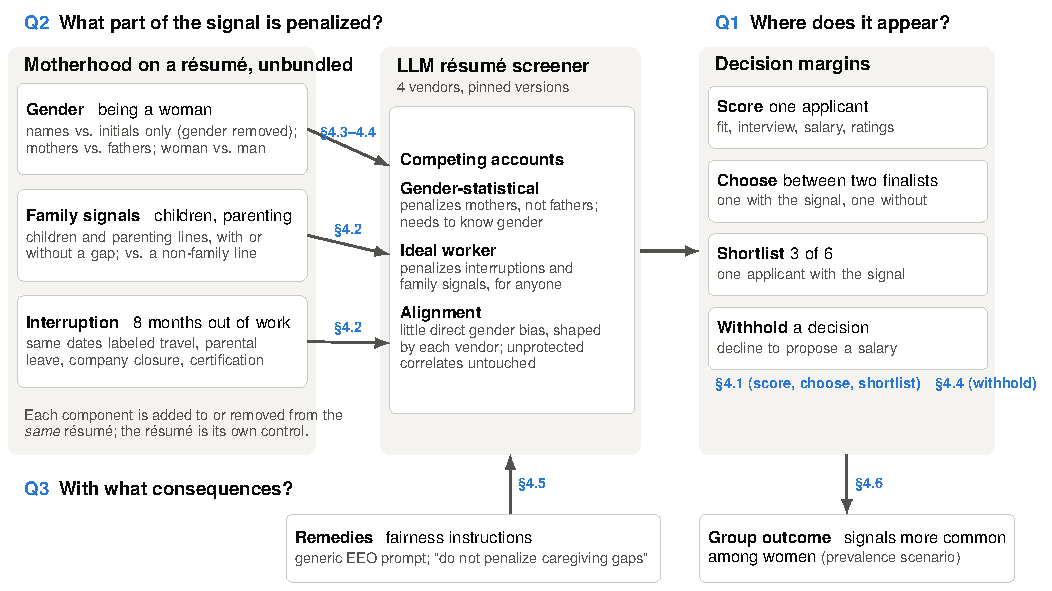
\includegraphics[width=1.0\textwidth]{figures/fig1_framework.pdf}
\caption{Framework: protection follows the label. Components of the motherhood signal are ordered by how directly they refer to a protected category, from named gender to correlated caregiving signals. Each column states the Study 1 test and what the label account expects; bands show where outcomes are measured, how remedies are tested, and the planned Study 2. Section numbers locate each test.}
\label{fig:framework}
\end{figure}

Study 1 tests these expectations in an audit of widely used models. It
unbundles the motherhood signal on identical résumés, varies how
directly gender is conveyed, observes the result at the decision margins
where selection happens, and tests the fairness instructions that
deployers commonly add. The findings line up with the gradient.
Caregiving signals carry a large penalty that falls on fathers as much
as on mothers, is unchanged when gender information is removed, and
appears only when applicants are compared. Explicitly named gender
elicits small and vendor-specific behavior---correction toward women in
one model, parity in another---rather than a penalty; a fourth model,
reported separately, responds with refusals. An instruction that names
caregiving gaps reduces the gap penalty but not the penalty on family
signals. Study 2, which we describe as a planned design, asks where the
gradient comes from by comparing the same open-weight model before and
after post-training.

The argument contributes to three conversations. For the sociology of
gender and work, it separates components of the motherhood penalty that
human hiring confounds and shows that, in these systems, the
ideal-worker components survive while the gendered one does not (Acker
1990; Williams 2000). For research on discrimination and its regulation,
it identifies a mechanism---protection that attaches to labels rather
than consequences---by which discrimination can persist through
correlated signals once a category is policed, a pattern with parallels
in studies of employers who lose access to a signal (Agan and Starr
2018). For algorithmic auditing, it shows that audits organized around
protected categories, single-applicant scores, or answered questions
only would certify these systems as fair.

\hypertarget{background}{%
\section{Background}\label{background}}

\hypertarget{the-motherhood-bundle}{%
\subsection{The motherhood bundle}\label{the-motherhood-bundle}}

Explanations of the motherhood penalty can be read as claims about which
part of the bundle does the work. \emph{Gender-statistical accounts}
hold that employers treat motherhood as a proxy for lower availability
and that the inference is gendered: mothers, not fathers, are expected
to reduce their commitment (Phelps 1972; Correll, Benard, and Paik
2007), and a normative variant holds that mothers violate expectations
of devotion to family (Benard and Correll 2010). Both predict a penalty
specific to mothers, which requires the evaluator to know the
applicant's gender. \emph{Ideal-worker accounts} locate the penalty in
the organization of work around an abstract worker who is fully
available and free of outside obligations (Acker 1990; Williams 2000;
Blair-Loy 2003). On this view the penalty attaches to departures from
continuous employment and to signs of competing obligations, whoever
shows them. Men who signal caregiving are penalized too (Rudman and
Mescher 2013; Williams, Blair-Loy, and Berdahl 2013), and employment
gaps are penalized whatever their reason (Kroft, Lange, and Notowidigdo
2013; Weisshaar 2018). Because women take most caregiving leaves (Goldin
2014), such a penalty is gendered in its consequences even when it is
not gendered in its application.

\hypertarget{alignment-and-the-label}{%
\subsection{Alignment and the label}\label{alignment-and-the-label}}

Commercial LLMs are trained after pretraining to follow instructions and
to produce outputs that raters and written principles prefer, including
outputs that do not treat people differently by protected attributes.
Audits of automated hiring have likewise asked mostly whether outcomes
differ by protected attributes signaled through names (An et al.~2025;
Armstrong et al.~2024; Rozado 2025; Wilson and Caliskan 2024), following
the logic of anti-discrimination law, which asks whether outcomes differ
across protected categories (Barocas and Selbst 2016). Both practices
are organized around the category. Neither directly targets signals that
are correlated with a category but not named by it. If models learn from
this kind of training to recognize and handle protected categories when
they are named, their behavior toward a signal should depend on how
directly it names one. Training against a category could produce
caution---equal treatment, correction in favor of the protected group,
or refusal---where the category is explicit, while leaving judgments
about correlated signals as pretraining left them.

\hypertarget{expectations-along-the-gradient}{%
\subsection{Expectations along the
gradient}\label{expectations-along-the-gradient}}

Figure 1 arranges the components of the motherhood signal by how
directly they refer to gender and states what the label account expects
at each position.

\begin{itemize}
\tightlist
\item
  \emph{Named gender} (an explicit ``Gender: Female/Male'' line):
  careful, developer-specific handling---parity, correction toward
  women, or refusal---rather than a penalty.
\item
  \emph{Implied gender} (a gendered first name): read, but acted on
  weakly; removing it should change little.
\item
  \emph{Correlated signals} (an employment gap; children and parenting
  activities): penalized, for anyone who carries them, as the
  ideal-worker account predicts.
\item
  \emph{Remedies}: an instruction protects the signal it names and not
  the ones it leaves unnamed.
\end{itemize}

The gender-statistical account makes contrary predictions: a penalty for
mothers but not fathers, which shrinks when gender is removed. The
framework also says where to look. Selection is comparative, and a
penalty that reflects relative judgments about availability may surface
only when applicants compete, so the expectations are tested at several
decision margins. We state these as orienting expectations; the tests
specified before data collection are listed in Section 3.4.

\hypertarget{study-1-design}{%
\section{Study 1: Design}\label{study-1-design}}

Study 1 is a correspondence-style audit (Bertrand and Mullainathan 2004)
of LLM screeners. Every estimate compares a résumé with itself, with and
without a signal, so applicant quality is held constant by construction.

\hypertarget{unbundling-the-correlated-signals}{%
\subsection{Unbundling the correlated
signals}\label{unbundling-the-correlated-signals}}

Table 1 lists the signals. Every application includes a short cover
note, so conditions differ only in what the note and résumé say. The
\emph{parent} signal adds ``married with two children'' to the note and
a parent-teacher association line to the résumé; \emph{parent with
leave} adds an eight-month ``Parental leave'' entry. Three placebos
separate the components: a \emph{travel gap} with the same dates
isolates the interruption; \emph{parental leave only}, without children,
isolates the caregiving label; and a length-matched \emph{personal} line
isolates disclosure. The comparisons yield four components: the
interruption (travel gap against equal treatment), its caregiving label
(parental leave only minus travel gap), family signals on top of a
labeled leave (parent with leave minus parental leave only), and
parenthood without a gap net of disclosure (parent minus personal).
Because travel might itself be stigmatized, a later phase substitutes
two neutral labels with the same dates (``Job search after company
closure,'' ``Full-time certification program''). \emph{Parent with
commitment evidence} and a \emph{pregnancy} signal, for women only,
complete the set. The signals are deliberately explicit; the
parental-leave gap is the most realistic and anchors the decomposition.

\begin{table}[tbp]
\centering\small
\caption{Unbundling the motherhood signal}\label{tab:cues}
\begin{tabularx}{\textwidth}{@{}l>{\raggedright\arraybackslash}X>{\raggedright\arraybackslash}X@{}}
\toprule
Signal & What it adds to the same résumé & What the comparison isolates \\
\midrule
None & neutral cover note & baseline \\
Personal (placebo) & a length-matched hobby and volunteer line & disclosure as such \\
Travel gap (placebo) & 8-month ``Career break --- extended travel'' & the interruption (vs.\ equal treatment) \\
Parental leave only (placebo) & the same dates labeled ``Parental leave'' & the caregiving label (vs.\ travel gap) \\
Parent & ``married with two children''; parent-association line & parenthood without a gap (vs.\ personal) \\
Parent + leave & Parent plus the parental-leave entry & family signals on top of a leave (vs.\ leave only) \\
\addlinespace
Neutral gap labels & same dates as ``company closure'' or ``certification'' & whether travel is stigmatized \\
Parent + commitment & Parent plus objective commitment bullets & the normative account \\
Pregnant (women only) & ``currently pregnant'' & pregnancy, incl.\ withholding \\
\bottomrule
\end{tabularx}
\begin{minipage}{\textwidth}\footnotesize\vspace{3pt}
\emph{Note:} Signals render identically for women and men; every application includes a cover note. Gender information is varied separately (names; name or initial plus an explicit gender line; initials only).
\end{minipage}
\end{table}

\hypertarget{moving-along-the-gradient-how-gender-is-conveyed}{%
\subsection{Moving along the gradient: how gender is
conveyed}\label{moving-along-the-gradient-how-gender-is-conveyed}}

Gender information is varied at four levels that correspond to positions
in Figure 1: the first name alone (implied); the name plus a header line
stating ``Gender: Female/Male'' (named); a gender-neutral initial plus
that line (named, without the name); and initials only (gender removed).
Names are six per gender from Bertrand and Mullainathan (2004), all
coded as White to hold race constant (Gaddis 2017), rotated within every
condition. Direct choices between a woman and a man with the same family
status measure gender preference as such. A perception check confirms
that models read implied gender: whenever a model used a gendered
pronoun in an explanation, it matched the name or header in every case,
and gendered pronouns all but disappeared under initials only. Asked
directly, however, models often answered ``unknown'' for names (Luna 34
percent, Haiku 58 percent) while stating explicit headers correctly in
every case---an early sign that what models \emph{say} about gender is
itself a trained behavior.

\hypertarget{decision-margins-and-remedies}{%
\subsection{Decision margins and
remedies}\label{decision-margins-and-remedies}}

Signals are evaluated at four margins: \emph{scoring} one applicant (fit
on a ten-point scale, interview recommendation, salary, four ratings);
\emph{choosing} between two finalists of the same gender, one with the
signal and one without (counterbalanced; equal treatment = 50 percent);
\emph{shortlisting} three of six applicants, one with the signal (impact
ratio relative to the same résumé without it, comparable to the
four-fifths rule); and \emph{declining to decide}---refusing or
withholding a salary---recorded as an outcome. A remedies phase repeats
the pairwise tasks under three system prompts: none, a generic
equal-employment-opportunity prompt, and that prompt plus ``do not
penalize employment gaps taken for caregiving,'' which names the gap but
not the family signals.

\hypertarget{models-materials-and-inference}{%
\subsection{Models, materials, and
inference}\label{models-materials-and-inference}}

We audited four widely available, low-cost models---DeepSeek V4.1 Flash,
GPT-6 Luna, Qwen 3.8 Flash, and Claude Haiku 5.5---pinned to dated
versions and single endpoints, with reasoning disabled, structured
output, and no system prompt except in the remedies phase. The main text
reports the first three. Claude Haiku's behavior differs in ways that
complicate comparison: it declines to choose or to propose a salary far
more often than the others, and its refusals are concentrated in exactly
the cells that carry family and gender signals, so its choice estimates
condition on answering in a way the others' do not. We therefore report
it separately and in full in Appendix A. This is a presentation decision
made after data collection; all pre-specified tests including Haiku are
in the replication report, and Haiku's penalties are larger than the
other models', so excluding it from the main text makes the reported
penalties conservative. The materials are 154 résumés validated as
qualified for 28 occupations, 20 spanning occupational female share (4.7
to 97.1 percent) and wages and 8 chosen to weaken the correlation
between female share and care work. Data were collected in four phases
between October 14 and 30, 2026 (616,419 logged calls).

Standard errors are clustered at the design's units: pairwise choices by
the unordered pair of résumés (40 pairs in the main occupations, 16 in
the added ones), scores by résumé, shortlists by occupation with résumé
and position fixed effects. Effective sample sizes are set by résumé
pairs, not calls. Tests use the Holm correction within families; claims
of no difference are tested for equivalence at ±5 percentage points;
few-cluster tests are checked with wild cluster bootstrap; and main
tests are re-estimated as linear probability models with controls.
Responses produced by repair passes are excluded from choice analyses,
and refusals and unusable answers are analyzed as outcomes and bounded
(Section 4.4). Designs and confirmatory tests were specified in analysis
plans committed before each paid run; the ±5-point bound for the second
phase was chosen after its data were collected but before the tests were
run, and was specified in advance for the remedies phase. The study was
not registered externally; other analyses are labeled exploratory, and
cross-model comparisons are descriptive.

\hypertarget{study-1-results}{%
\section{Study 1: Results}\label{study-1-results}}

We report results for DeepSeek, Luna, and Qwen; Claude Haiku is reported
separately in Appendix A (Section 3.4 explains why). We begin at the
correlated end of the gradient, where the label account expects the
largest effects, then move to named gender, to remedies, and to
variation across occupations. Differences are in percentage points
(``points'').

\hypertarget{correlated-signals-a-caregiver-penalty}{%
\subsection{Correlated signals: a caregiver
penalty}\label{correlated-signals-a-caregiver-penalty}}

\emph{It appears where selection happens.} Family signals barely move
the scores models give a single applicant: relative to the same résumé
without the signal, the parent signals change women's fit ratings by at
most 0.35 points on a ten-point scale and interview recommendations by
at most 1.5 percentage points. When applicants compete, the same signals
are costly (Table 2). A mother returning from parental leave is chosen
against an equally qualified childless woman 31 percent of the time by
DeepSeek, 23 by Qwen, and 19 by Luna, against 50 percent under equal
treatment. In shortlisting, mothers reach the shortlist at 71, 75, and
78 percent of their childless rate, each below the four-fifths
threshold. Choices are not magnified scores. Choices respond to ordinary
differences in résumé quality at 13 to 18 points per fit point; by that
yardstick the family signals act like quality losses of 0.8 to 2.0 fit
points, 3.6 to 34 times their actual effect on scores. A noise model
built from each model's own rating variability predicts much smaller
penalties than observed in five of six model-signal combinations, by 7
to 18 points (Figure 2); the exception is DeepSeek's leave signal, whose
choice penalty matches its score penalty.

\begin{table}[tbp]
\centering\small
\begin{threeparttable}
\caption{Probability that the applicant with the family signal is chosen in pairwise choice (main run)}\label{tab:choice}
\begin{tabular}{@{}lccc@{}}
\toprule
Signal --- applicant & DeepSeek & Luna & Qwen \\
\midrule
Parent --- mother & .357 & .297 & .387 \\
Parent --- father & .349 & .294 & .398 \\
Parent + commitment --- mother & .419 & .228 & .407 \\
Parent + leave --- mother & .310 & .186 & .230 \\
Parent + leave --- father & .308 & .184 & .256 \\
\midrule
\multicolumn{4}{@{}l}{\emph{Shortlisting: rate relative to the same résumé without the signal}} \\
Mothers & .71 & .78 & .75 \\
Fathers & .70 & .81 & .80 \\
\bottomrule
\end{tabular}
\begin{tablenotes}\footnotesize
\item \emph{Note:} Pairwise choice against an equally qualified childless candidate of the same gender; .50 = equal treatment. 95\% confidence intervals clustered by résumé pair (40 pairs) are $\pm$.02--.07; none includes .50. Shortlisting ratios are résumé fixed-effect estimates from pools of six; .80 is the four-fifths threshold. Claude Haiku: Table A1.
\end{tablenotes}
\end{threeparttable}
\end{table}

\begin{figure}[tbp]
\centering
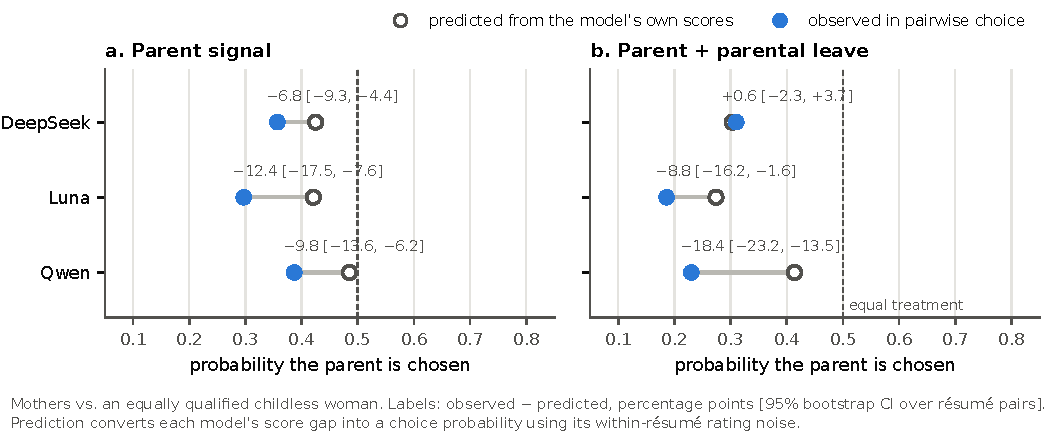
\includegraphics[width=1.0\textwidth]{figures/fig2_scores_vs_choices.pdf}
\caption{The caregiver penalty appears where selection happens. Hollow markers: probability that a mother is chosen over an equally qualified childless woman, predicted from the model's own scores; filled markers: observed.}
\label{fig:scores}
\end{figure}

\emph{It consists of the interruption and the family signals, not the
label.} Table 3 and Figure 3 decompose the parent-with-leave penalty
(mothers, explicit gender, 40 résumé pairs). An eight-month gap labeled
travel costs 10.5 (DeepSeek) to 26.0 points (Luna). Calling the same gap
parental leave adds nothing: it is 1.7 to 6.6 points \emph{less} costly
than travel. Travel was not unusually stigmatized. When it was replaced
by company closure or certification, no neutral label was significantly
more costly than travel after correction; Qwen penalized travel 4.3 to
5.4 points more than either neutral label; and the largest estimate in
the other direction was DeepSeek's certification label for women (4.0
points, Holm p = .14). Adding children and parenting activity to a
résumé that already carries a labeled leave costs a further 10.7 to 12.3
points, and parenthood without a gap, net of the personal placebo, costs
8.0 to 12.1 points. The personal placebo itself costs only 2.7 to 3.5
points. Commitment evidence does not restore equal treatment: it raises
mothers' choice share modestly for DeepSeek and Qwen and lowers it for
Luna (Table 2).

\begin{table}[tbp]
\centering\small
\begin{threeparttable}
\caption{Placebo decomposition of the parent-with-leave penalty (percentage points)}\label{tab:decomp}
\begin{tabular}{@{}lccc@{}}
\toprule
Component (comparison) & DeepSeek & Luna & Qwen \\
\midrule
Interruption & $-10.5$ & $-26.0$ & $-22.1$ \\
\quad(travel gap vs.\ .50) & ($t=-8.0$) & ($t=-7.3$) & ($t=-8.8$) \\
Caregiving label & $+1.7$ & $+6.5$ & $+6.6$ \\
\quad(parental leave only $-$ travel gap) & [$+0.5$, $+2.9$] & [$+3.7$, $+9.2$] & [$+4.8$, $+8.4$] \\
Family signals on top of leave & $-10.7$ & $-11.5$ & $-12.3$ \\
\quad(parent + leave $-$ parental leave only) & [$-12.7$, $-8.6$] & [$-15.4$, $-7.5$] & [$-14.8$, $-9.8$] \\
Parenthood net of disclosure & $-10.4$ & $-12.1$ & $-8.0$ \\
\quad(parent $-$ personal placebo) & [$-12.8$, $-8.0$] & [$-16.3$, $-7.9$] & [$-11.1$, $-4.9$] \\
\bottomrule
\end{tabular}
\begin{tablenotes}\footnotesize
\item \emph{Note:} Mothers; 20 main occupations; gender stated explicitly (levels L1 and L2 pooled); 40 résumé pairs. Brackets: 95\% confidence intervals clustered by résumé pair. The personal placebo itself costs 2.7--3.5 points.
\end{tablenotes}
\end{threeparttable}
\end{table}

\begin{figure}[tbp]
\centering
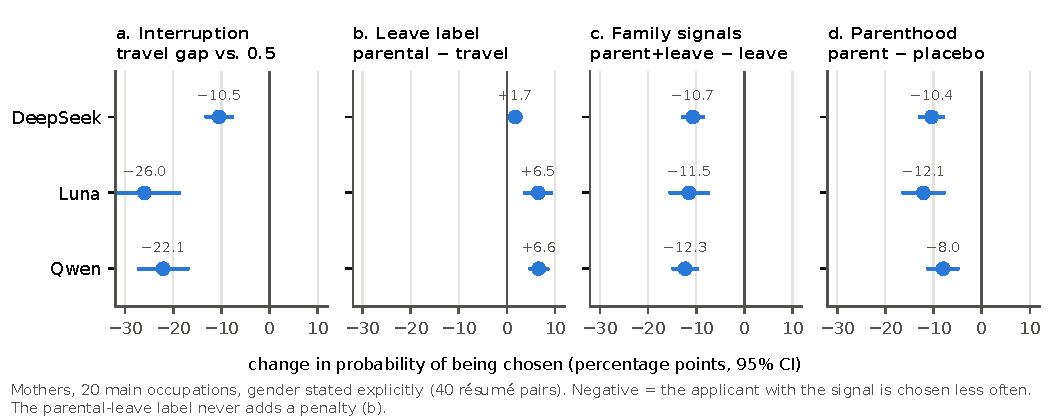
\includegraphics[width=1.0\textwidth]{figures/fig3_decomposition.pdf}
\caption{Decomposition of the parent-with-leave penalty: the interruption and family signals carry it; the caregiving label adds nothing.}
\label{fig:decomp}
\end{figure}

\emph{It does not depend on gender.} Figure 4 asks what happens when the
model can no longer know the applicant's gender. In the added
occupations, the parent penalty with gendered names and the penalty
under initials only are almost identical (panel a): they differ by +0.6
(DeepSeek), −1.3 (Luna), and +0.7 points (Qwen). Because a
nonsignificant difference could simply reflect low power, we test
equivalence (panel b): in five of six model-signal combinations the 90
percent interval lies inside ±5 points, so the difference is
statistically equivalent to zero; in the sixth, DeepSeek's leave signal,
it reaches 5.6. The design could detect differences of 3.0 to 5.4
points. The absence of a difference is the result: removing gender
leaves the penalty intact. Fathers tell the same story. They are chosen
below equal treatment in every cell---a father returning from leave is
chosen 31, 26, and 18 percent of the time by DeepSeek, Qwen, and
Luna---and there is no fatherhood bonus. Mother--father differences in
choice are within 2.6 points and not significant after correction in any
of the three models (Table 4).

\begin{figure}[tbp]
\centering
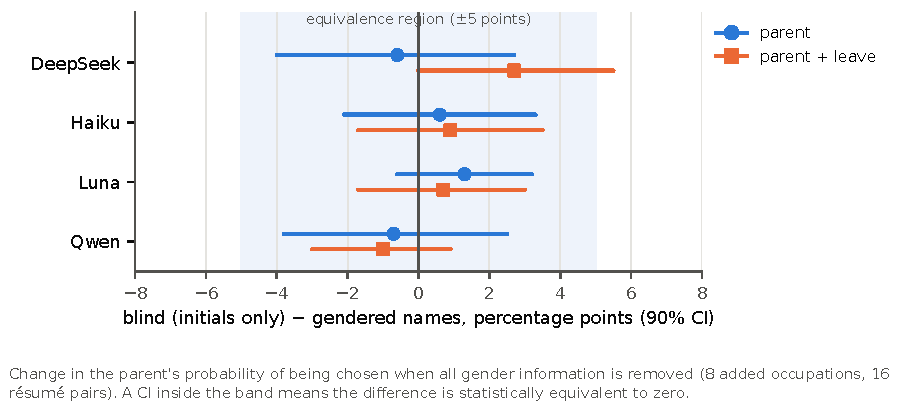
\includegraphics[width=1.0\textwidth]{figures/fig5_invariance.pdf}
\caption{Removing all gender information leaves the penalty unchanged. (a) Probability the parent is chosen when gender is conveyed by name and when it is removed. (b) The difference with its 90\% confidence interval; intervals inside the shaded band are statistically equivalent to zero. A null difference here is the finding.}
\label{fig:invariance}
\end{figure}

\begin{table}[tbp]
\centering\small
\begin{threeparttable}
\caption{Mother--father differences (main run)}\label{tab:mf}
\begin{tabular}{@{}llccc@{}}
\toprule
Signal & Outcome & DeepSeek & Luna & Qwen \\
\midrule
Parent & Pairwise choice (points) & $+0.8$ & $-0.4$ & $-1.1$ \\
 & Paired salary (\$) & $+118$ & $-100$ & $-456$ \\
 & Commitment, single applicant & $\mathbf{-.09}$ & $+.03$ & $-.00$ \\
Parent + leave & Pairwise choice (points) & $+0.2$ & $+0.2$ & $-2.6$ \\
 & Paired salary (\$) & $+72$ & $-9$ & $-543$ \\
 & Commitment, single applicant & $\mathbf{-.12}$ & $+.01$ & $-.04$ \\
\bottomrule
\end{tabular}
\begin{tablenotes}\footnotesize
\item \emph{Note:} Mother minus father on the same résumé pairs (choice, salary) or résumés (single-applicant ratings, 1--7 scale). Bold: significant after Holm correction within outcome. No choice difference is significant.
\end{tablenotes}
\end{threeparttable}
\end{table}

\emph{The models' explanations follow the decomposition (exploratory).}
In LLM-coded explanations of pairwise choices (DeepSeek V4.1 Flash
coder; Qwen 3.8 Flash second coder; κ = .71 to .93 for the six codes
used, lower for availability and family on explanations not written by
DeepSeek), the gap was cited in 24 to 88 percent of losses for the gap
signals and in at most 1 percent for parent signals without a gap;
family was cited for parent signals (12 to 64 percent) but never for the
travel gap or the personal placebo; and all pre-stated contrasts
survived Holm correction (Supplementary Figure S1). For DeepSeek and
Qwen, explanations called family information irrelevant much more often
when the parent lost than when the parent won (53 vs.~19 and 90 vs.~42
percent). These are stated justifications, coded without human
validation, not causes.

At the correlated end of the gradient, then, the models apply a
caregiver penalty: a penalty on time out of work and on visible family
responsibility, shared by all three models, borne by women and men
alike.

\hypertarget{named-gender-careful-vendor-specific-handling}{%
\subsection{Named gender: careful, vendor-specific
handling}\label{named-gender-careful-vendor-specific-handling}}

At the named end, the label account expects careful handling rather than
a penalty, shaped by each developer. In direct choices between a woman
and a man with the same family status (Table 5, Figure 5), none of the
three models penalizes women, and naming gender explicitly changes their
behavior in model-specific ways. Luna's mild preference for women under
names (.522 childless, .577 parents) grows with an explicit gender line
(.587 and .647). DeepSeek shows a small, stable preference for women
(.535 to .548 for mothers). Qwen stays within five points of parity at
every level, as equivalence tests confirm (its largest deviation is a
1.8-point tilt toward childless women under initials). Explicit gender
fields are therefore not neutral: they activate corrections toward women
in one model and leave another at parity. Refusals were almost absent in
these three models (DeepSeek and Luna essentially never refused; Qwen's
missing answers were formatting failures, not refusals). Caution
expressed as refusal and withholding is concentrated in Claude Haiku
(Appendix A).

\begin{table}[tbp]
\centering\small
\begin{threeparttable}
\caption{Direct woman-versus-man choices: probability the woman is chosen}\label{tab:direct}
\begin{tabular}{@{}llccc@{}}
\toprule
Model & Pair & Names (L0) & Name + line (L1) & Initial + line (L2) \\
\midrule
DeepSeek & childless / parents & .514 / \textbf{.535} & \textbf{.540} / \textbf{.540} & \textbf{.538} / \textbf{.548} \\
Luna & childless / parents & \textbf{.522} / \textbf{.577} & \textbf{.587} / \textbf{.647} & \textbf{.575} / \textbf{.634} \\
Qwen & childless / parents & .505 / .504 & .494 / .515 & \textbf{.518} / .493 \\
\bottomrule
\end{tabular}
\begin{tablenotes}\footnotesize
\item \emph{Note:} Both candidates share a family status; .50 = no preference; 56 résumé pairs. Bold: differs from .50 after Holm correction (six tests per model). Qwen is statistically equivalent to .50 within $\pm$5 points in every cell.
\end{tablenotes}
\end{threeparttable}
\end{table}

\begin{figure}[tbp]
\centering
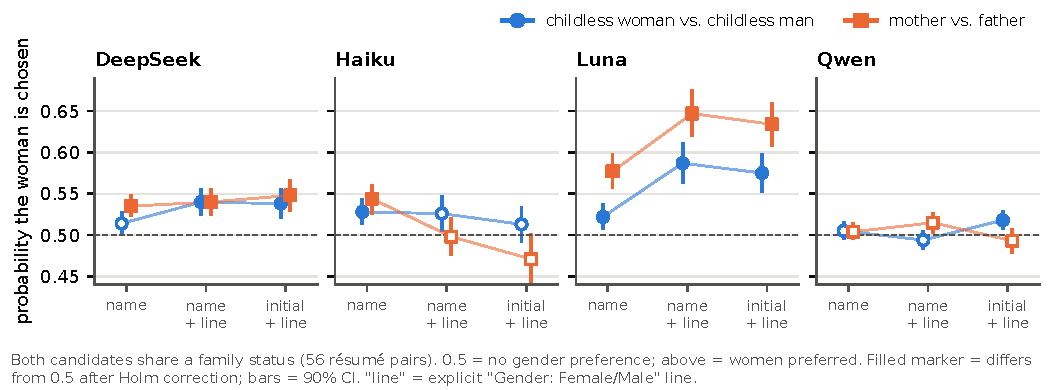
\includegraphics[width=0.9\textwidth]{figures/fig6_direct_gender.pdf}
\caption{Named gender: direct woman-versus-man choices by how gender is conveyed.}
\label{fig:direct}
\end{figure}

\hypertarget{remedies-an-instruction-protects-what-it-names}{%
\subsection{Remedies: an instruction protects what it
names}\label{remedies-an-instruction-protects-what-it-names}}

Table 6 reports the remedies phase (48,000 calls). A generic
equal-opportunity prompt, which names gender but not caregiving, left
the caregiver penalty in place, with effects that depended on the
vendor: no significant change for DeepSeek, a reduction of the plain
parent penalty for Luna (5.0 points) but not of the leave penalty, and a
\emph{deepening} of both penalties for Qwen (4.7 and 5.3 points). Adding
``do not penalize employment gaps taken for caregiving'' reduced the
penalty for the parent with leave--- the signal the sentence names---by
4.5 to 9.1 points relative to no system prompt, and the plain parent
penalty, which carries no gap, did not change significantly after
correction. Relative to the generic prompt, the added sentence raised
the leave cell by 8.5 to 9.8 points but the plain parent cell by only
1.8 to 4.4 (Table 6). No arm reached equal treatment. Named gender
behavior responded readily: Luna's preference for mothers over fathers
fell from .640 to .557 under the generic prompt. Naming a signal moved
it toward protection; leaving it unnamed did not.

\begin{table}[tbp]
\centering\small
\begin{threeparttable}
\caption{Fairness instructions (remedies phase): probability that a mother is chosen, by system prompt}\label{tab:fair}
\begin{tabular}{@{}lccc@{}}
\toprule
Model & Parent & Parent + leave & Travel gap \\
\midrule
DeepSeek & .361 / .325 / .369 & .317 / .301 / .386 & .422 / .420 / .451 \\
Luna & .307 / .357 / .376 & .195 / .188 / .286 & .238 / .283 / .307 \\
Qwen & .381 / .333 / .351 & .234 / .181 / .279 & .274 / .286 / .339 \\
\bottomrule
\end{tabular}
\begin{tablenotes}\footnotesize
\item \emph{Note:} Entries: no system prompt / generic equal-opportunity prompt / generic prompt plus ``do not penalize employment gaps taken for caregiving.'' Women; 20 main occupations; 40 résumé pairs; .50 = equal treatment. Hypotheses and tests were specified before the run. Claude Haiku: Table A1.
\end{tablenotes}
\end{threeparttable}
\end{table}

\hypertarget{occupations-a-penalty-everywhere-weakly-patterned}{%
\subsection{Occupations: a penalty everywhere, weakly
patterned}\label{occupations-a-penalty-everywhere-weakly-patterned}}

Occupations differ in how gendered they are and in how much they involve
care, and the design included both kinds of variation: 20 occupations
spanning female share from 4.7 to 97.1 percent, and 8 chosen to separate
female share from care work. If models had learned occupation-specific
stereotypes---mothers as less suited to male-dominated or demanding
jobs---the penalty should vary systematically with these attributes. It
does not vary much. Regressing the leave penalty for mothers on
occupational female share and care intensity across the 28 occupations,
the coefficient on female share is positive in all three models (mothers
fare slightly better in more female-dominated occupations: +.057 for
DeepSeek, +.048 for Luna, +.028 for Qwen, per standard deviation), but
only DeepSeek's is nominally significant (p = .024), and none survives
correction for the 18 tests in this family; care intensity is negative
for DeepSeek and Luna and positive for Qwen, nominally significant only
for Luna (p = .050). The caregiver penalty is thus a general feature of
how the models evaluate applicants, not a product of occupational
stereotyping. Occupation-level estimates are in Supplementary Figure S2
(pending).

\hypertarget{robustness}{%
\subsection{Robustness}\label{robustness}}

Missing answers cannot explain the penalty. Even if every missing choice
had gone to the parent, worst-case bounds leave every headline cell
below equal treatment (for the mother with leave in the main run, at
most .32 for DeepSeek, .22 for Luna, and .39 for Qwen, whose wider bound
reflects its higher rate of unparseable output, itself higher in parent
cells). Linear probability models with controls reproduce the main
tests; wild cluster bootstrap p-values change no conclusion; and
estimates drifted little between phases. Supplementary results: paired
salary offers are about 2 percent lower for mothers; ``greedy''
availability language in job ads adds to the leave penalty for DeepSeek
mothers (2.7 points) and, combined with family-friendly language, for
DeepSeek applicants of both genders (5.2 and 6.0 points), while
family-friendly language alone never helps.

\hypertarget{study-2-planned-where-does-the-gradient-come-from}{%
\section{Study 2 (planned): Where does the gradient come
from?}\label{study-2-planned-where-does-the-gradient-come-from}}

Study 1 shows that behavior lines up with the gradient; it cannot show
that alignment produced it. The four audited models are aligned
commercial systems without unaligned counterparts, and their developers'
training choices are not observed. Study 2 tests the mechanism directly
by holding the model fixed and varying only its stage of training.

\emph{Models.} Open-weight model families that release checkpoints from
successive training stages---a pretrained base model, an
instruction-tuned model, and a preference-tuned model---allow the same
network to be compared before and after each stage (for example, the
OLMo family, which publishes its post-training checkpoints and data). We
will use two or more such families, at sizes that run on a single 80GB
GPU, so that conclusions do not rest on one developer.

\emph{Measurement.} Base models do not reliably follow instructions or
produce structured output. We therefore measure choices from the models'
probabilities rather than their text: for each pairwise prompt, the
log-probability of answering ``A'' versus ``B,'' averaged over both
orderings of the candidates. The same quantity is computed for every
checkpoint, so stages are compared on one scale. The Study 1 materials
and conditions are reused: the placebo ladder at the correlated end,
names versus initials at the implied position, and explicit gender lines
and direct woman-versus-man pairs at the named end.

\emph{Predictions.} If protection follows the label because of
alignment, then (1) named gender effects should be present in base
models and shrink, or reverse toward women, after instruction and
preference tuning; (2) the caregiver penalty should be present at every
stage and change little; and (3) the gap between the named and
correlated ends should widen across stages. Evidence against the account
would be a caregiver penalty that emerges only after alignment, or
named-gender effects that are already absent in base models.

\emph{Extension.} Because the models are open, Study 2 can also ask what
changes inside them: whether the representation of gender that a model
forms from a résumé differs across training stages, and whether
caregiving signals activate that representation. Steering experiments
that suppress or amplify a gender direction would test whether the
caregiver penalty depends on it.

\hypertarget{discussion}{%
\section{Discussion}\label{discussion}}

\hypertarget{the-framework-revisited}{%
\subsection{The framework revisited}\label{the-framework-revisited}}

Figure 6 returns to the framework with Study 1's findings in place. At
the correlated end, caregiving signals carry a large penalty for anyone
who shows them. At the implied position, models read gender but act on
it little: removing it changes nothing. At the named end, gender elicits
small and vendor-specific handling---correction or parity, and in Claude
Haiku refusal---rather than a penalty. And an instruction protects what
it names. The gender-statistical account, which places the penalty on
mothers as women, does not fit; the ideal-worker account describes the
penalty that remains; and the label account describes why the remaining
penalty takes the form it does.

\begin{figure}[tbp]
\centering
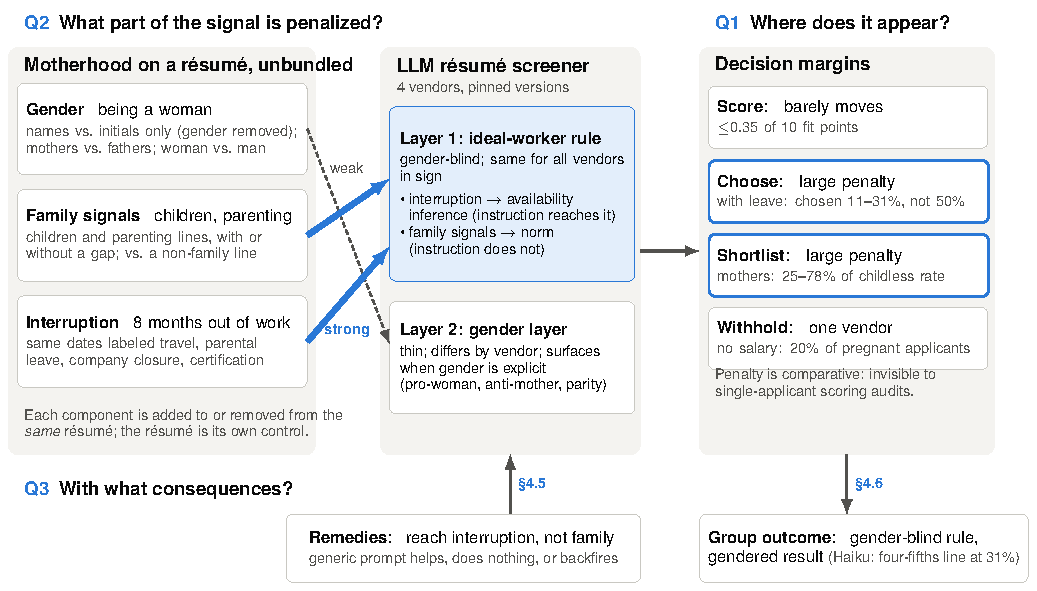
\includegraphics[width=1.0\textwidth]{figures/fig9_findings.pdf}
\caption{The framework revisited with Study 1's findings in place.}
\label{fig:findings}
\end{figure}

The caregiver penalty itself has two parts with different characters.
The interruption penalty behaves like an inference about availability
(Phelps 1972; Kroft, Lange, and Notowidigdo 2013; Weisshaar 2018): any
gap is costly whatever it is called, availability language deepens it,
and naming it in an instruction reduces it. The family-signal penalty
behaves like a norm: it attaches to children and parenting activity,
persists on top of a gap already labeled as parental leave, is not
offset by evidence of commitment, and does not respond to
instructions---like the normative component of the human motherhood
penalty (Benard and Correll 2010), except that it is applied to fathers
too.

\hypertarget{gender-neutral-in-form-gendered-in-effect}{%
\subsection{Gender-neutral in form, gendered in
effect}\label{gender-neutral-in-form-gendered-in-effect}}

Protection that follows the label leaves the consequences of correlated
signals unprotected. Caregiving interruptions and visible family
responsibilities are carried disproportionately by women (Goldin 2014),
so a rule that penalizes them reproduces a gender gap through the
distribution of signals rather than the treatment of individuals. Figure
7 shows how this happens: applying each model's measured shortlisting
penalty to pools in which more women than men carry a caregiving signal,
the women-to-men shortlisting ratio falls below the four-fifths line
once more than 73 (DeepSeek), 84 (Qwen), or 93 percent (Luna) of women
carry the signal, with men at 5 percent. These thresholds are high
because these three models' shortlisting penalties are moderate; for
Claude Haiku, whose penalty is far larger, the threshold is 31 percent
(Appendix A). Prevalence is a scenario parameter here, but the structure
is the one disparate-impact doctrine was designed to capture, and the
one the ideal-worker literature has long described: a norm that
disadvantages women without naming them (Acker 1990; Williams 2000).

\begin{figure}[tbp]
\centering
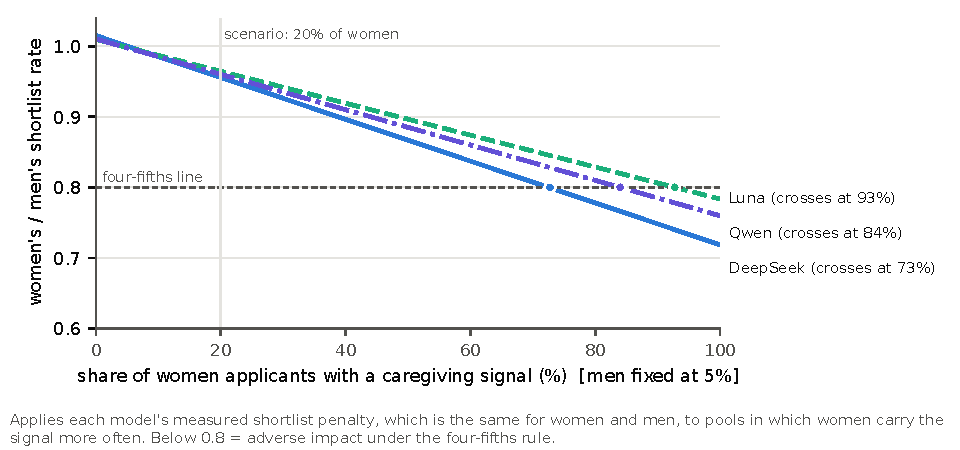
\includegraphics[width=0.9\textwidth]{figures/fig8_disparate_impact.pdf}
\caption{Gender-neutral in form, gendered in effect: implied ratio of women's to men's shortlist rates as women's prevalence of caregiving signals rises (men fixed at 5\%).}
\label{fig:di}
\end{figure}

The broader implication concerns how discrimination responds to its
regulation. When a protected category is policed, decisions can continue
through correlated signals that are not protected as such, as research
on bans of criminal-record questions has shown (Agan and Starr 2018).
Alignment adds a twist: here the system itself has been trained around
the category, and that training appears to make it attentive to how a
signal is labeled rather than to what the signal does.

\hypertarget{implications-for-auditing}{%
\subsection{Implications for auditing}\label{implications-for-auditing}}

The framework explains why standard audits would miss these patterns.
Audits keyed to protected categories compare women and men and find
little; they need to compare applicants with and without caregiving
signals. Audits that score single applicants find small effects; the
penalty lives in choices and shortlists. Audits that drop non-answers
miss the largest pregnancy effect, a refusal to price that carries a
denial of interviews. And audits that ask models about gender measure
what models are willing to say, not what they use. For deployers, the
remedies phase cautions that fairness instructions protect what they
name and can backfire for some vendors.

\hypertarget{limitations}{%
\subsection{Limitations}\label{limitations}}

The family signals are explicit, and real résumés carry weaker ones. The
materials are US-oriented, English, text-only, and hold race constant.
Pregnancy has no male counterpart. Outcomes are recommendations, not
offers or callbacks. The models are four low-cost versions at fixed
dates; larger models and commercial products may differ. Pools and pairs
are constructed, so the design identifies the effect of a signal, not
hiring rates. The disparate-impact analysis uses scenario prevalence
values. The coding of explanations relies on LLM coders without human
validation. Effective sample sizes are set by résumé pairs (40 or 16 per
comparison). Above all, Study 1 shows that behavior is consistent with
the label account; Study 2 is needed to show that alignment produces it.

\hypertarget{a-research-agenda}{%
\section{A Research Agenda}\label{a-research-agenda}}

The label account generates questions beyond this paper. We list those
we consider most informative, roughly in order of how directly they test
the account.

\begin{enumerate}
\def\labelenumi{\arabic{enumi}.}
\tightlist
\item
  \emph{Rewording the signal.} If protection follows the label, wording
  that names a protected category should be treated differently from
  wording that does not, even when the underlying fact is the same.
  Candidate contrasts: ``maternity leave'' and ``paternity leave''
  versus ``parental leave''; ``pregnancy leave'' versus ``medical
  leave''; gender-coded activities (a women's sports team, a sorority)
  versus neutral ones.
\item
  \emph{Other protected categories along the same gradient.} Age offers
  a clean test: stated age (named) versus graduation year (correlated);
  disability: ``disability leave'' versus ``medical leave'' versus an
  unexplained gap; race: stated race versus names versus neighborhoods
  or institutions. The account predicts the same ordering in each case.
\item
  \emph{Refusal as an outcome.} Where and why models decline to
  decide---by category, by explicitness, and by vendor---and what
  happens to applicants they decline.
\item
  \emph{Representations and steering.} In open models, whether
  caregiving signals activate internal gender representations, how
  alignment changes those representations, and whether steering them
  changes decisions (Study 2 extension).
\item
  \emph{Human comparison.} The same unbundling design with human
  evaluators, to compare which components humans and models penalize on
  identical materials---the clearest way to say whether models
  reproduce, transform, or exceed the human penalty.
\item
  \emph{Realistic signals and deployed systems.} Weaker, naturally
  phrased caregiving signals; larger models; commercial screening
  products with their own system prompts; and other labor markets and
  languages, including markets in which explicit gender and age fields
  are standard.
\item
  \emph{Group consequences with real prevalence.} Estimates of how often
  women and men applicants carry caregiving signals, from household
  surveys, to turn the disparate-impact scenario into an estimate.
\end{enumerate}

\hypertarget{conclusion}{%
\section{Conclusion}\label{conclusion}}

Asked whether LLM résumé screeners penalize mothers, Study 1's answer is
that the models we studied penalize caregivers. They penalize time out
of work and visible family responsibility regardless of gender, and only
when applicants are compared, while handling explicitly named gender
with care that differs from vendor to vendor. We have argued that this
is what protection that follows the label looks like: systems trained
around a protected category treat the category carefully and its
correlates freely. Because the correlates of motherhood are carried
mostly by women, such systems can pass fairness checks organized around
gender while reproducing the motherhood penalty in effect. Whether
alignment is the cause is the question Study 2 is designed to answer.

\hypertarget{appendix-a.-claude-haiku}{%
\section{Appendix A. Claude Haiku}\label{appendix-a.-claude-haiku}}

\setcounter{figure}{0}\renewcommand{\thefigure}{A\arabic{figure}}\setcounter{table}{0}\renewcommand{\thetable}{A\arabic{table}}

Claude Haiku 5.5 was audited with the same materials and procedures as
the other models. We report it separately because two features of its
behavior complicate comparison. First, it declines to decide far more
often, and selectively: in the second phase it refused to choose in 5.4
percent of mother-versus-father comparisons, 4.9 percent of
parent-with-leave comparisons, and 2.7 percent of plain parent
comparisons, against about 0.1 percent for the placebo signals (refusals
were more frequent for women than for men in every cell), and it
withheld any salary for 19.8 percent of pregnant applicants (3.1 percent
for childless women), 27.5 percent when gender was stated explicitly
(Figure A1). Second, its scores and choices point in opposite
directions: it rates mothers 0.34 points \emph{higher} than the same
applicants without children, yet chooses them far less often.

\begin{table}[tbp]
\centering\small
\begin{threeparttable}
\caption{Claude Haiku: main results}\label{tab:haiku}
\begin{tabular}{@{}lr@{}}
\toprule
Quantity & Estimate \\
\midrule
Pairwise choice, parent + leave: mother / father & .110 / .130 \\
Pairwise choice, parent: mother / father & .233 / .276 \\
Shortlisting ratio: mothers / fathers & .25 / .23 \\
Fit rating, parent $-$ none (women; 10-point scale) & $+0.34$ \\
Interruption (travel gap vs.\ .50), points & $-18.4$ ($t=-8.5$) \\
Caregiving label, points & $-1.1$ [$-3.2$, $+0.9$] \\
Family signals on top of leave, points & $-17.4$ [$-20.2$, $-14.5$] \\
Parenthood net of disclosure, points & $-19.2$ [$-23.4$, $-15.0$] \\
Personal placebo, points & $+3.7$ \\
No gender $-$ names: parent / parent + leave, points & $+0.6$ / $+0.9$ (both equivalent) \\
Mother $-$ father choice, parent, points & $-4.3$ (Holm $p=.02$) \\
Direct choice, mother vs.\ father: L0 / L1 / L2 & .544 / .498 / .471 \\
Refusal to choose: mother vs.\ father / parent + leave / placebos & 5.4\% / 4.9\% / $\approx$0.1\% \\
Salary withheld: pregnant / childless women (L1: pregnant) & 19.8\% / 3.1\% (27.5\%) \\
Interview if offer withheld vs.\ made (pregnant) & 29.9\% vs.\ 100\% \\
Generic prompt: change in parent / leave penalty & $+6.6$ / $+12.2$ points \\
Four-fifths threshold (women's signal prevalence; men 5\%) & 31\% \\
\bottomrule
\end{tabular}
\begin{tablenotes}\footnotesize
\item \emph{Note:} Same designs and clustering as the main tables. Refusal rates from the second phase, first attempts.
\end{tablenotes}
\end{threeparttable}
\end{table}

\begin{figure}[tbp]
\centering
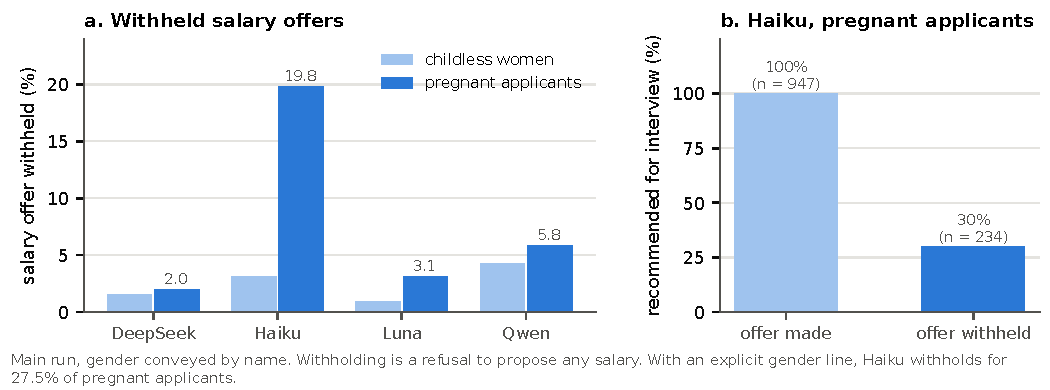
\includegraphics[width=1.0\textwidth]{figures/figA1_withholding.pdf}
\caption{Claude Haiku: salary offers withheld by model (a) and interview recommendations for Haiku's pregnant applicants by whether an offer was made (b).}
\label{fig:withhold}
\end{figure}

Selective refusal means Haiku's choice estimates condition on answering.
Worst-case bounds show that refusals cannot explain its penalty: if
every refused choice had gone to the parent, the mother with leave would
still be chosen at most about 13 percent of the time in the main run.
With that caveat, Haiku shows the caregiver penalty in its strongest
form (Table A1). A mother returning from leave is chosen 11 percent of
the time against a childless woman, a father 13 percent; mothers are
shortlisted at 25 percent of their childless rate. In the decomposition,
the travel gap costs 18.4 points; the parental label is statistically
equivalent to zero; family signals on top of a labeled leave cost 17.4
points; parenthood net of disclosure costs 19.2 points; and the personal
placebo slightly \emph{helps} (3.7 points). Removing gender leaves the
penalty unchanged (both differences equivalent to zero within ±5
points). Haiku is the only model with a mother-specific penalty: it
chooses mothers 4.3 points less often than fathers (Holm p = .02) and
rates them lower on commitment.

At the named end, Haiku's slight preference for mothers under names
(.544) disappears when gender is stated explicitly (.498; .471 with
initials), and together with its refusals and its pregnancy withholding
this is the clearest instance of caution around named gender in the
data. Caution, however, is not equal treatment: pregnant applicants
without a salary offer were recommended for interview 29.9 percent of
the time, against every time when an offer was made, a net interview
penalty of 9.4 points relative to childless women. Fairness instructions
also worked differently for Haiku: the generic prompt reduced its
penalties substantially (6.6 and 12.2 points), and it is the only model
whose family-signal penalty fell under the targeted instruction. Because
its shortlisting penalty is large, its gender-blind rule produces a
four-fifths violation once more than 31 percent of women carry a
caregiving signal.

Haiku therefore strengthens rather than weakens the main conclusions: it
shows the largest caregiver penalty, no dependence on gender
information, and the most pronounced caution where gender is named.
Whether its distinctive profile reflects its developer's training
choices cannot be determined from these data; Study 2 is designed to
address that kind of question.

\section*{References}
{\small\setstretch{1.1}
\noindent\textit{Items marked ◆ are to be checked against the source before submission;
items marked † were added in the manuscript and are not yet in the
report's verified list.}\par\medskip
\noindent\hangindent=1.5em\hangafter=1 Acker, Joan. 1990. ``Hierarchies, Jobs, Bodies: A Theory of Gendered
Organizations.'' \emph{Gender \& Society} 4(2):139--158.\par\smallskip
\noindent\hangindent=1.5em\hangafter=1 Agan, Amanda, and Sonja Starr. 2018. ``Ban the Box, Criminal Records,
and Racial Discrimination: A Field Experiment.'' \emph{Quarterly Journal
of Economics} 133(1):191--235. †\par\smallskip
\noindent\hangindent=1.5em\hangafter=1 An, Jiafu, Difang Huang, Chen Lin, and Mingzhu Tai. 2025. ``Measuring
Gender and Racial Biases in Large Language Models: Intersectional
Evidence from Automated Resume Evaluation.'' \emph{PNAS Nexus}
4(3):pgaf089.\par\smallskip
\noindent\hangindent=1.5em\hangafter=1 Armstrong, Lena, Abbie Liu, Stephen MacNeil, and Danaë Metaxa. 2024.
``The Silicon Ceiling: Auditing GPT's Race and Gender Biases in
Hiring.'' arXiv:2405.04412.\par\smallskip
\noindent\hangindent=1.5em\hangafter=1 Barocas, Solon, and Andrew D. Selbst. 2016. ``Big Data's Disparate
Impact.'' \emph{California Law Review} 104(3):671--732. †\par\smallskip
\noindent\hangindent=1.5em\hangafter=1 Benard, Stephen, and Shelley J. Correll. 2010. ``Normative
Discrimination and the Motherhood Penalty.'' \emph{Gender \& Society}
24(5):616--646.\par\smallskip
\noindent\hangindent=1.5em\hangafter=1 Bertrand, Marianne, and Sendhil Mullainathan. 2004. ``Are Emily and Greg
More Employable than Lakisha and Jamal?'' \emph{American Economic
Review} 94(4):991--1013.\par\smallskip
\noindent\hangindent=1.5em\hangafter=1 Blair-Loy, Mary. 2003. \emph{Competing Devotions: Career and Family
among Women Executives}. Cambridge, MA: Harvard University Press. †\par\smallskip
\noindent\hangindent=1.5em\hangafter=1 Budig, Michelle J., and Paula England. 2001. ``The Wage Penalty for
Motherhood.'' \emph{American Sociological Review} 66(2):204--225. †\par\smallskip
\noindent\hangindent=1.5em\hangafter=1 Correll, Shelley J., Stephen Benard, and In Paik. 2007. ``Getting a Job:
Is There a Motherhood Penalty?'' \emph{American Journal of Sociology}
112(5):1297--1338.\par\smallskip
\noindent\hangindent=1.5em\hangafter=1 EEOC. 1978. Uniform Guidelines on Employee Selection Procedures. 43 FR
38290.\par\smallskip
\noindent\hangindent=1.5em\hangafter=1 European Union. 2024. Regulation (EU) 2024/1689 (Artificial Intelligence
Act).\par\smallskip
\noindent\hangindent=1.5em\hangafter=1 Frermann, Lea, Sheilla Njoto, Marc Cheong, and Leah Ruppanner. 2023.
``Gender Bias and Parental-Leave Gaps in ChatGPT Résumé Ranking.''
University of Melbourne. ◆\par\smallskip
\noindent\hangindent=1.5em\hangafter=1 Gaddis, S. Michael. 2017. ``How Black Are Lakisha and Jamal? Racial
Perceptions from Names Used in Correspondence Audit Studies.''
\emph{Sociological Science} 4:469--489.\par\smallskip
\noindent\hangindent=1.5em\hangafter=1 Goldin, Claudia. 2014. ``A Grand Gender Convergence: Its Last Chapter.''
\emph{American Economic Review} 104(4):1091--1119. †\par\smallskip
\noindent\hangindent=1.5em\hangafter=1 Kroft, Kory, Fabian Lange, and Matthew J. Notowidigdo. 2013. ``Duration
Dependence and Labor Market Conditions: Evidence from a Field
Experiment.'' \emph{Quarterly Journal of Economics} 128(3):1123--1167.\par\smallskip
\noindent\hangindent=1.5em\hangafter=1 Phelps, Edmund S. 1972. ``The Statistical Theory of Racism and Sexism.''
\emph{American Economic Review} 62(4):659--661. ◆\par\smallskip
\noindent\hangindent=1.5em\hangafter=1 Rozado, David. 2025. ``Gender and Positional Biases in LLM-Based Hiring
Decisions.'' arXiv:2505.17049.\par\smallskip
\noindent\hangindent=1.5em\hangafter=1 Rudman, Laurie A., and Kris Mescher. 2013. ``Penalizing Men Who Request
a Family Leave: Is Flexibility Stigma a Femininity Stigma?''
\emph{Journal of Social Issues} 69(2):322--340.\par\smallskip
\noindent\hangindent=1.5em\hangafter=1 Veldanda, Akshaj Kumar, et al.~2023. ``Investigating Algorithmic Hiring
Bias in the Era of ChatGPT.'' arXiv:2310.05135. ◆\par\smallskip
\noindent\hangindent=1.5em\hangafter=1 Weisshaar, Katherine. 2018. ``From Opt Out to Blocked Out: The
Challenges for Labor Market Re-entry after Family-Related Employment
Lapses.'' \emph{American Sociological Review} 83(1):34--60.\par\smallskip
\noindent\hangindent=1.5em\hangafter=1 Williams, Joan C. 2000. \emph{Unbending Gender: Why Family and Work
Conflict and What to Do About It}. New York: Oxford University Press.\par\smallskip
\noindent\hangindent=1.5em\hangafter=1 Williams, Joan C., Mary Blair-Loy, and Jennifer L. Berdahl. 2013.
``Cultural Schemas, Social Class, and the Flexibility Stigma.''
\emph{Journal of Social Issues} 69(2):209--234.\par\smallskip
\noindent\hangindent=1.5em\hangafter=1 Wilson, Kyra, and Aylin Caliskan. 2024. ``Gender, Race, and
Intersectional Bias in Resume Screening via Language Model Retrieval.''
AIES.\par\smallskip
\noindent\hangindent=1.5em\hangafter=1 Yin, Leon, Davey Alba, and Leonardo Nicoletti. 2024. ``OpenAI's GPT Is a
Recruiter's Dream Tool. Tests Show There's Racial Bias.''
\emph{Bloomberg}.\par\smallskip}
\end{document}
